% Provenance (never printed): cycle 4 SVT, "La planete Terre, l'environnement
% et l'action humaine": natural risks, hazard and vulnerability, prevention
% and protection; see sources/book1/PROVENANCE.md. Book 1, grade 9, chapter 2.
% Vocabulary guard: owns risk, vulnerability, prevention, hazard map.
% Natural hazard and natural disaster, the warning colours and the safety
% rules are g5's (natural-hazards); the warning signs of an eruption and the
% Pinatubo story are g7's (volcanoes); seismometer, tsunami and "scientists
% cannot predict earthquakes" are g7's (earthquakes); flood and floodplain
% are g5's (water-shapes-the-land); weather forecast is g8's. Lahars are
% called mudflows (as in g7). "Normal fault" is Book 2's: here "a fault".
\chapter{Conviver com os riscos naturais}\label{ch:g9:natural-risks}

Na noite de 13~de~novembro de 1985, a maior parte dos moradores de
Armero, uma cidade da Colômbia, estava na cama. Uma \omterm{def:g5:natural-hazards:storm}{tempestade} escondia o
\omterm{def:g4:volcanoes-earthquakes-first-look:volcano}{vulcão} nevado Nevado del Ruiz, a \qty{45}{km} dali, e ninguém na cidade o
viu entrar em \omterm{def:g4:volcanoes-earthquakes-first-look:eruption}{erupção}. As \omterm{def:g3:stones-pebbles-sand:rock}{rochas} quentes derreteram parte do seu gelo, e a
água, misturada com cinzas e \omterm{def:g3:stones-pebbles-sand:rock}{rochas}, desceu os \omterm{def:g1:landscapes-around-us:landform}{vales} como fluxos de lama.
Cerca de duas horas depois, os fluxos de lama saíram do \omterm{def:g1:landscapes-around-us:landform}{vale} do \omterm{def:g1:landscapes-around-us:water}{rio}
Lagunillas, direto sobre a cidade: cerca de \num{23000} pessoas, a maior
parte da cidade, morreram. Duas horas eram tempo suficiente para ir a pé
até um terreno mais alto. Os moradores de Armero não foram avisados.
% ledger: usgs:armero

\begin{omfigure}
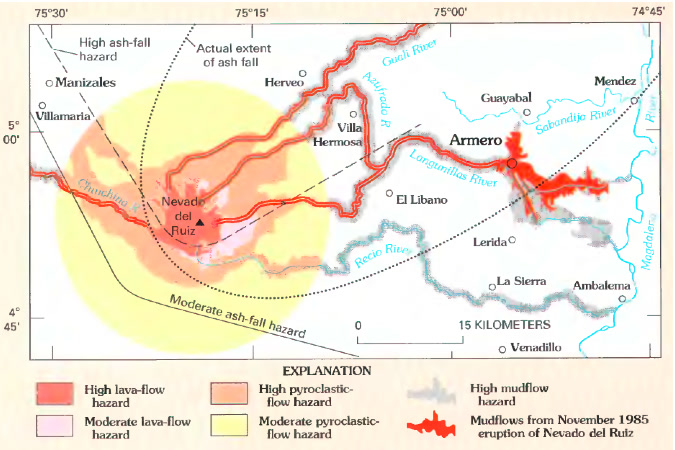
\includegraphics[width=0.86\linewidth]{images/book1/g9-ruiz-hazard-map.jpg}

{\small O \omterm{def:g9:natural-risks:hazard-map}{mapa de ameaças} do Nevado del Ruiz. Uma primeira versão,
desenhada por geólogos colombianos, circulou um mês antes da \omterm{def:g4:volcanoes-earthquakes-first-look:eruption}{erupção} e já
mostrava o perigo de fluxos de lama no \omterm{def:g1:landscapes-around-us:landform}{vale} de Armero. Esta versão,
redesenhada depois do desastre, acrescenta em vermelho vivo os fluxos de
lama que realmente vieram em novembro de 1985 (o círculo sombreado em
volta do \omterm{def:g4:volcanoes-earthquakes-first-look:volcano}{vulcão} tem um raio de cerca de \qty{20}{km}). De T.~L.~Wright e
T.~C.~Pierson, USGS Circular 1073, 1992 (domínio público, via Wikimedia
Commons).}
% ledger: usgs:ruiz-map, commons:ruiz-map
\label{fig:g9:natural-risks:ruiz}
\end{omfigure}

Seis anos depois, no monte Pinatubo, nas Filipinas, o \omterm{def:g4:volcanoes-earthquakes-first-look:volcano}{vulcão} estava sendo
vigiado, o alerta veio a tempo e as pessoas saíram
(\cref{ch:g7:volcanoes}). Os dois eram \omterm{def:g4:volcanoes-earthquakes-first-look:volcano}{vulcões} explosivos, com pessoas
morando no caminho dos seus fluxos de lama. O que mudou foi o que as
pessoas sabiam, e o que fizeram com isso. Este capítulo
trata dessa diferença.
% ledger: usgs:armero (Pinatubo 1991 averted a disaster like Armero), usgs:pinatubo-1991

\begin{recall}
Uma \emph{\omterm{def:g5:natural-hazards:hazard}{ameaça natural}} é um acontecimento natural que pode causar dano
às pessoas; ela se torna um \emph{\omterm{def:g5:natural-hazards:disaster}{desastre natural}} quando atinge um lugar
onde as pessoas vivem e causa grandes danos
(\cref{ch:g5:natural-hazards}). Um \omterm{def:g1:landscapes-around-us:water}{rio} que transborda cobre a sua
\omterm{def:g5:water-shapes-the-land:flood}{planície de inundação} (\cref{ch:g5:water-shapes-the-land}). Um \omterm{def:g4:volcanoes-earthquakes-first-look:volcano}{vulcão}
costuma dar sinais de alerta antes de uma grande \omterm{def:g4:volcanoes-earthquakes-first-look:eruption}{erupção}: pequenos
\omterm{def:g4:volcanoes-earthquakes-first-look:earthquake}{terremotos}, encostas que incham, gases (\cref{ch:g7:volcanoes}). Os
cientistas não conseguem prever os \omterm{def:g4:volcanoes-earthquakes-first-look:earthquake}{terremotos}; os \omterm{def:g7:earthquakes:seismometer}{sismômetros} os
registram, e um \omterm{def:g4:volcanoes-earthquakes-first-look:earthquake}{terremoto} embaixo do \omterm{def:g2:water-on-earth:ocean}{mar} pode provocar um \omterm{def:g7:earthquakes:tsunami}{tsunami}
(\cref{ch:g7:earthquakes}). Uma \omterm{def:g8:fronts-and-weather-maps:forecast}{previsão do tempo} diz como vai estar o
\omterm{def:g1:watching-the-weather:weather}{tempo} nos próximos dias (\cref{ch:g8:fronts-and-weather-maps}).
\end{recall}

\section{Ameaça, vulnerabilidade e risco}

O mesmo \omterm{def:g4:volcanoes-earthquakes-first-look:earthquake}{terremoto} não causa o mesmo dano em toda parte. Embaixo de um
\omterm{def:g5:weather-and-climate:desert}{deserto} vazio, ele não fere ninguém. Embaixo de uma cidade de prédios
sólidos, cujos moradores sabem o que fazer, ele sacode, assusta e quebra
janelas. Embaixo de uma cidade de casas pesadas e mal construídas, ele
pode derrubá-las sobre as pessoas que estão dentro. A ameaça é a mesma; o
que muda é a facilidade com que o lugar pode ser atingido.

\begin{definition}[Vulnerabilidade]\label{def:g9:natural-risks:vulnerability}
A \emph{vulnerabilidade}\index{vulnerabilidade} de um lugar é a
facilidade com que os seus moradores, os seus prédios e as coisas de que
eles precisam podem ser atingidos por uma \omterm{def:g5:natural-hazards:hazard}{ameaça natural}. Casas numa
\omterm{def:g5:water-shapes-the-land:flood}{planície de inundação}, prédios frágeis, nenhum alerta e nenhum plano
tornam um lugar vulnerável.
\end{definition}

\begin{definition}[Risco]\label{def:g9:natural-risks:risk}
O \emph{risco}\index{risco} que um lugar corre diante de uma \omterm{def:g5:natural-hazards:hazard}{ameaça
natural} é o perigo de dano aos seus moradores e aos seus bens. Ele
depende ao mesmo tempo da ameaça, da sua força e da sua frequência, e da
\omterm{def:g9:natural-risks:vulnerability}{vulnerabilidade} do lugar: onde não há ameaça, ou nada que possa ser
atingido, não há risco.
\end{definition}

\begin{omfigure}
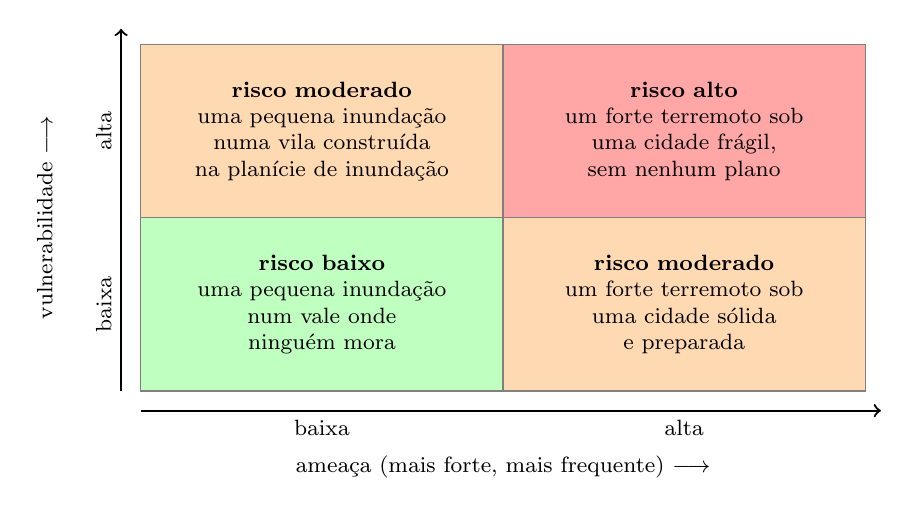
\begin{tikzpicture}[x=1cm, y=1cm, font=\footnotesize,
    cell/.style={minimum width=4.6cm, minimum height=2.2cm, align=center, draw=black!50, text width=4.2cm}]
  \node[cell, fill=green!25] at (2.3,1.1) {\textbf{risco baixo}\\ uma pequena inundação\\ num vale onde\\ ninguém mora};
  \node[cell, fill=orange!30] at (6.9,1.1) {\textbf{risco moderado}\\ um forte terremoto sob\\ uma cidade sólida\\ e preparada};
  \node[cell, fill=orange!30] at (2.3,3.3) {\textbf{risco moderado}\\ uma pequena inundação\\ numa vila construída\\ na planície de inundação};
  \node[cell, fill=red!35] at (6.9,3.3) {\textbf{risco alto}\\ um forte terremoto sob\\ uma cidade frágil,\\ sem nenhum plano};
  \draw[->, thick] (0,-0.25) -- (9.4,-0.25);
  \draw[->, thick] (-0.25,0) -- (-0.25,4.6);
  \node[anchor=north] at (4.6,-0.7) {ameaça (mais forte, mais frequente) $\longrightarrow$};
  \node[rotate=90, anchor=south] at (-1.0,2.2) {vulnerabilidade $\longrightarrow$};
  \node[below] at (2.3,-0.25) {baixa};
  \node[below] at (6.9,-0.25) {alta};
  \node[left] at (-0.25,1.1) {\rotatebox{90}{baixa}};
  \node[left] at (-0.25,3.3) {\rotatebox{90}{alta}};
\end{tikzpicture}

{\small A grade do \omterm{def:g9:natural-risks:risk}{risco} (um esboço). O \omterm{def:g9:natural-risks:risk}{risco} cresce com a ameaça e com a
\omterm{def:g9:natural-risks:vulnerability}{vulnerabilidade}. Mudar uma cidade de lugar raramente é possível, e não
dá para desligar uma ameaça; mas a \omterm{def:g9:natural-risks:vulnerability}{vulnerabilidade} da cidade pode ser
reduzida, o que faz a cidade descer na grade.}
\label{fig:g9:natural-risks:grid}
\end{omfigure}

Armero era um lugar de ameaça alta: um \omterm{def:g4:volcanoes-earthquakes-first-look:volcano}{vulcão} nevado que tinha despertado
um ano antes, e uma cidade construída sobre os depósitos de antigos
fluxos de lama, na saída de um \omterm{def:g1:landscapes-around-us:landform}{vale} que já os tinha levado antes. Era
também muito vulnerável: faltavam instrumentos e apoio aos cientistas, as
informações dadas às autoridades eram muitas vezes vagas, e não existia
nenhum plano de evacuação nem nenhum meio rápido de avisar a cidade.
% ledger: usgs:armero

\section{Previsão e prevenção}

Algumas ameaças podem ser vistas chegando. Uma \omterm{def:g5:natural-hazards:storm}{tempestade} é prevista com
dias de antecedência (\cref{ch:g8:fronts-and-weather-maps}); uma
\omterm{def:g5:water-shapes-the-land:flood}{inundação} depois de uma \omterm{def:g4:clouds-rain-snow:precipitation}{chuva} forte, com horas ou dias; uma grande
\omterm{def:g4:volcanoes-earthquakes-first-look:eruption}{erupção} muitas vezes se anuncia com dias ou semanas de antecedência,
embora nem sempre. Um \omterm{def:g7:earthquakes:tsunami}{tsunami} atravessa um \omterm{def:g2:water-on-earth:ocean}{oceano} em horas, então um
alerta pode chegar a \omterm{def:g1:landscapes-around-us:water}{litorais} distantes antes dele. Já os \omterm{def:g4:volcanoes-earthquakes-first-look:earthquake}{terremotos} não
podem ser previstos: os cientistas podem dizer quais \omterm{def:g7:earthquakes:fault}{falhas} vão se romper
de novo um dia, nunca em que dia.
% ledger: nws:tsunami-speed, usgs:eq-basics, usgs:pinatubo-1991

Uma previsão, por melhor que seja, só é útil se algo for feito antes de
a ameaça chegar. A maior parte desse trabalho é feita muito antes de
qualquer alerta.

\begin{definition}[Prevenção]\label{def:g9:natural-risks:prevention}
A \emph{prevenção}\index{prevencao@prevenção} é tudo o que se faz antes
de uma \omterm{def:g5:natural-hazards:hazard}{ameaça natural} chegar para reduzir o \omterm{def:g9:natural-risks:risk}{risco}: saber onde a ameaça
pode atingir, construir em lugares seguros e de maneira segura, vigiar a
ameaça, avisar as pessoas e prepará-las.
\end{definition}

A \omterm{def:g9:natural-risks:prevention}{prevenção} age nos dois lados da grade do \omterm{def:g9:natural-risks:risk}{risco}. Vigiar um \omterm{def:g4:volcanoes-earthquakes-first-look:volcano}{vulcão} ou um
\omterm{def:g1:landscapes-around-us:water}{rio} não o torna menos perigoso, mas dá tempo para agir. Construir longe
da \omterm{def:g5:water-shapes-the-land:flood}{planície de inundação}, construir casas sólidas, planejar os caminhos
até um terreno mais alto e treiná-los: tudo isso reduz a \omterm{def:g9:natural-risks:vulnerability}{vulnerabilidade}.

\begin{omfigure}
\begin{minipage}[c]{0.44\linewidth}\centering
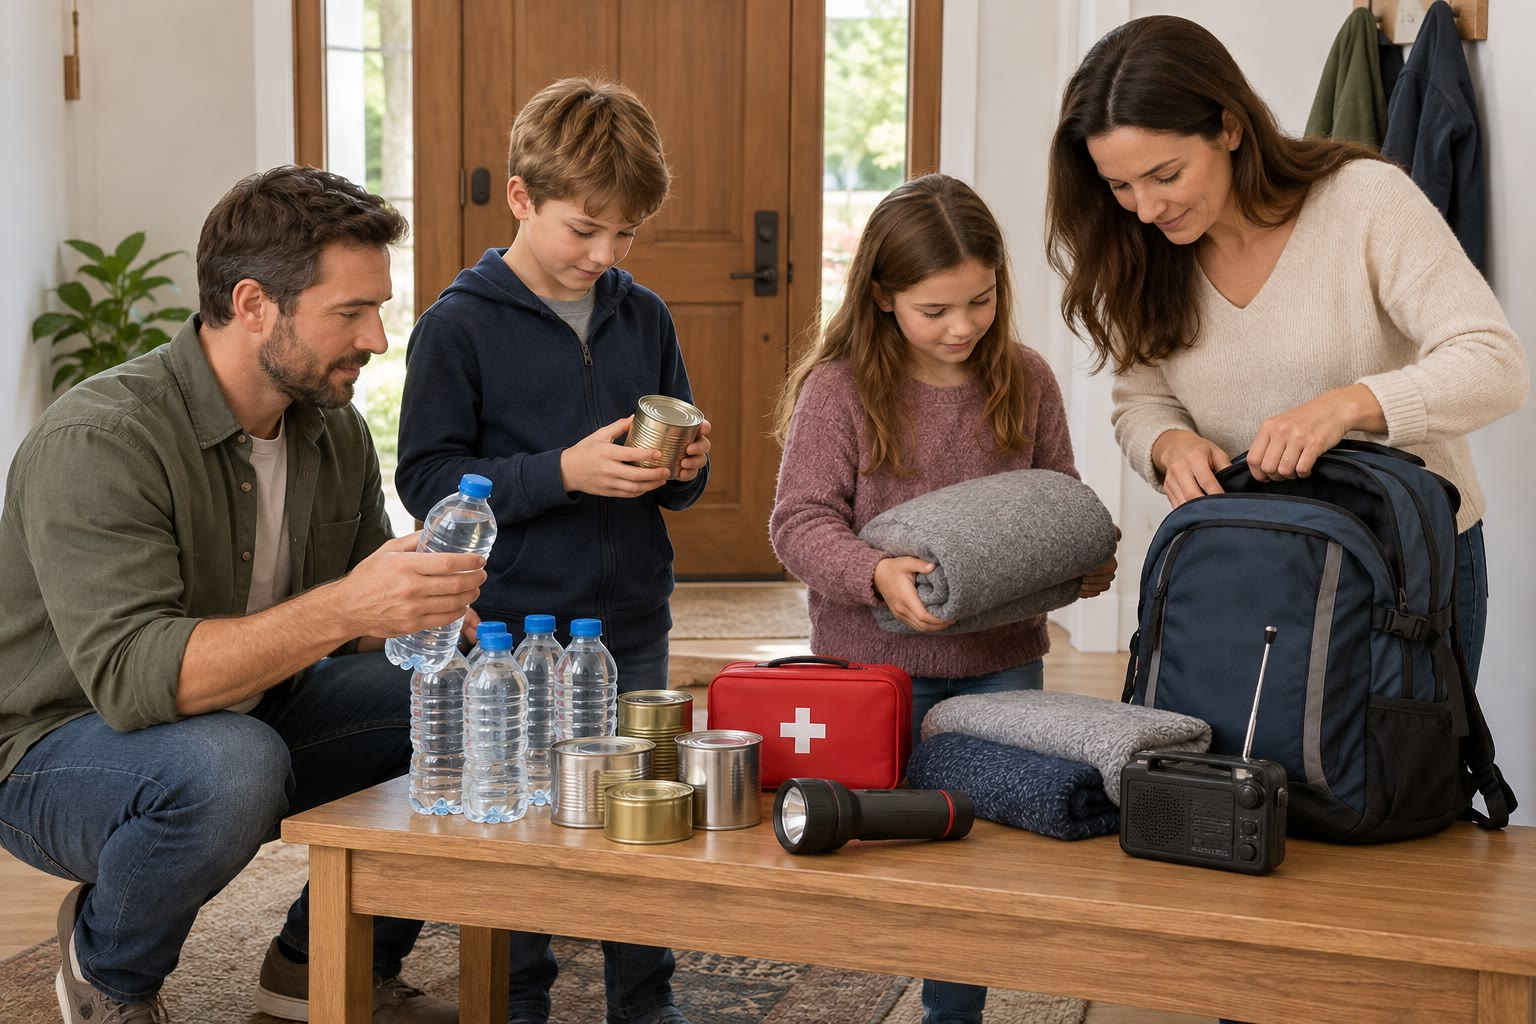
\includegraphics[width=\linewidth]{images/book1/ai/g9-emergency-kit.jpg}
\end{minipage}\hfill
\begin{minipage}[c]{0.52\linewidth}\raggedright
{\small Estar preparado: uma família confere o seu kit de emergência,
guardado perto da porta, pronto para ser levado se for preciso sair
depressa: água e comida que se conservam por vários dias, uma lanterna,
um rádio que funciona sem a rede elétrica, pilhas de reserva, um kit de
primeiros socorros e cobertores quentes (ilustração gerada por IA de uma
cena genérica).}
\end{minipage}
% ledger: ready:kit
\label{fig:g9:natural-risks:kit}
\end{omfigure}

\section{Vigiar os vulcões e as falhas}

Um observatório vulcanológico vigia os sinais de alerta do
\cref{ch:g7:volcanoes} com instrumentos que funcionam dia e noite e
enviam as suas medidas ao observatório.
% ledger: usgs:hvo-toolkit

\begin{omfigure}
\begin{tikzpicture}[x=1cm, y=1cm, font=\footnotesize, >={Stealth[length=2mm]}]
  % ground and cone
  \fill[black!13] (0,0) -- (0,1.0) -- (3.0,1.2) -- (5.4,3.6) -- (6.4,3.6) -- (8.8,1.2) -- (12,1.0) -- (12,0) -- cycle;
  \draw[black!60] (0,1.0) -- (3.0,1.2) -- (5.4,3.6) -- (6.4,3.6) -- (8.8,1.2) -- (12,1.0);
  % magma chamber and conduit
  \fill[omWarm!70] (5.9,0.6) ellipse (1.5 and 0.38);
  \fill[omWarm!70] (5.75,0.9) rectangle (6.05,3.6);
  \node[white, font=\scriptsize\bfseries] at (5.9,0.58) {magma};
  % gas plume, drifting west
  \fill[black!10] (5.8,3.95) circle (0.3) (5.35,4.35) circle (0.4) (4.75,4.75) circle (0.45);
  % swollen east flank, dashed
  \draw[dashed, omWarm, line width=0.8pt] (6.45,3.7) .. controls (7.5,3.55) and (8.6,2.6) .. (8.85,1.25);
  \draw[->, omWarm] (7.3,2.75) -- (7.7,3.15);
  \node[anchor=west, align=left, text=omWarm!80!black] at (8.2,3.75) {o magma que sobe\\ incha a encosta};
  % tiltmeter on the east flank
  \fill[black] (7.75,2.12) rectangle (8.05,2.24);
  \draw[black!70] (8.1,2.2) -- (8.5,2.45);
  \node[anchor=west, align=left] at (8.5,2.55) {inclinômetro: a encosta\\ se inclina ao inchar};
  % GPS receiver on the west flank, and its satellite
  \draw[black, line width=0.6pt] (4.4,2.6) -- (4.4,2.95);
  \fill[black] (4.25,2.95) rectangle (4.55,3.05);
  \draw[black] (4.4,3.05) circle (0.1);
  \draw[black, fill=white] (1.7,4.85) rectangle (2.0,5.05);
  \draw[black] (1.4,4.95) -- (2.3,4.95);
  \node[anchor=east] at (1.35,4.95) {satélite};
  \draw[black!50, dashed] (4.3,3.15) -- (2.05,4.8);
  \draw[black!70] (3.05,2.65) -- (4.2,2.85);
  \node[anchor=east, align=right] at (3.0,2.6) {receptor GPS: o\\ chão se move\\ milímetros};
  % gas instrument on the crater rim
  \fill[black] (6.45,3.6) rectangle (6.75,3.75);
  \draw[black!70] (6.8,3.75) -- (7.1,4.45);
  \node[anchor=west, align=left] at (7.1,4.6) {medidor de gases: os gases\\ que escapam da cratera};
  % seismometer (in the ground)
  \fill[black] (2.1,0.95) rectangle (2.4,1.1);
  \node[anchor=north, align=center] at (1.6,0.85) {sismômetro:\\ pequenos terremotos};
  % camera, east, looking at the summit
  \fill[black] (10.7,1.12) rectangle (11.0,1.32);
  \fill[black] (10.7,1.17) -- (10.55,1.12) -- (10.55,1.32) -- (10.7,1.27) -- cycle;
  \node[anchor=north, align=center] at (10.8,0.85) {câmera:\\ vigia o cume};
\end{tikzpicture}

{\small Vigiar um \omterm{def:g4:volcanoes-earthquakes-first-look:volcano}{vulcão} (um esboço, fora de escala). Os \omterm{def:g7:earthquakes:seismometer}{sismômetros}
contam os pequenos \omterm{def:g4:volcanoes-earthquakes-first-look:earthquake}{terremotos}; os inclinômetros e os receptores GPS,
presos à \omterm{def:g3:stones-pebbles-sand:rock}{rocha}, medem como o chão se inclina e se move à medida que o
\omterm{def:g7:volcanoes:magma}{magma} se acumula embaixo; outros instrumentos medem os gases que
escapam; câmeras vigiam o cume. \omterm{def:g4:clouds-rain-snow:rain-gauge}{Pluviômetros} ajudam a distinguir os
sinais do \omterm{def:g4:volcanoes-earthquakes-first-look:volcano}{vulcão} dos efeitos de uma \omterm{def:g4:clouds-rain-snow:precipitation}{chuva} forte.}
% ledger: usgs:hvo-toolkit
\label{fig:g9:natural-risks:monitoring}
\end{omfigure}

Nenhum desses sinais dá o dia e a hora de uma \omterm{def:g4:volcanoes-earthquakes-first-look:eruption}{erupção}. Os cientistas os
leem em conjunto, como um médico lê várias medidas de um paciente, e
dizem como o perigo muda; as autoridades decidem quando fechar uma área e
quando retirar as pessoas. No Pinatubo, essa corrente funcionou. No
Nevado del Ruiz, o \omterm{def:g4:volcanoes-earthquakes-first-look:volcano}{vulcão} dava sinais havia um ano, com enxames de
\omterm{def:g4:volcanoes-earthquakes-first-look:earthquake}{terremotos}, mas os instrumentos eram poucos, e a corrente que ia dos
cientistas aos moradores de Armero estava rompida.
% ledger: usgs:armero, usgs:hvo-toolkit, usgs:pinatubo-1991

As \omterm{def:g7:earthquakes:fault}{falhas} são vigiadas da mesma maneira, por redes de \omterm{def:g7:earthquakes:seismometer}{sismômetros} e de
estações GPS que medem, milímetro por milímetro, como os dois lados de
uma \omterm{def:g7:earthquakes:fault}{falha} se movem lentamente. Isso indica quais \omterm{def:g7:earthquakes:fault}{falhas} estão acumulando
a tensão do próximo grande \omterm{def:g4:volcanoes-earthquakes-first-look:earthquake}{terremoto}, mas não quando ele virá. Para os
\omterm{def:g4:volcanoes-earthquakes-first-look:earthquake}{terremotos}, a \omterm{def:g9:natural-risks:prevention}{prevenção} é a principal defesa.
% ledger: usgs:gps, usgs:eq-basics

\section{Mapas de ameaças e zonas de inundação}

O primeiro passo da \omterm{def:g9:natural-risks:prevention}{prevenção} é saber onde uma ameaça pode atingir.

\begin{definition}[Mapa de ameaças]\label{def:g9:natural-risks:hazard-map}
Um \emph{mapa de ameaças}\index{mapa de ameacas@mapa de ameaças} mostra
os lugares que uma \omterm{def:g5:natural-hazards:hazard}{ameaça natural} pode alcançar, muitas vezes com vários
níveis de perigo. Ele é desenhado a partir do que a ameaça fez no passado
e da forma do terreno.
\end{definition}

O \omterm{def:g2:drawing-to-map:map}{mapa} do Nevado del Ruiz, no início deste capítulo, é um \omterm{def:g9:natural-risks:hazard-map}{mapa de
ameaças}: os fluxos de lama do passado tinham seguido os \omterm{def:g1:landscapes-around-us:landform}{vales}, e os
próximos também os seguiriam. Os \omterm{def:g2:drawing-to-map:map}{mapas} de \omterm{def:g5:water-shapes-the-land:flood}{inundação} seguem a mesma ideia.
A água se espalha pelo terreno baixo e plano ao lado de um \omterm{def:g1:landscapes-around-us:water}{rio}: quanto
mais alta a \omterm{def:g5:water-shapes-the-land:flood}{inundação}, mais larga a faixa de terreno que ela cobre. Um
\omterm{def:g2:drawing-to-map:map}{mapa} de \omterm{def:g5:water-shapes-the-land:flood}{inundação} desenha a borda da água para uma \omterm{def:g5:water-shapes-the-land:flood}{inundação} escolhida,
muitas vezes a \omterm{def:g5:water-shapes-the-land:flood}{inundação} que tem uma chance de 1 em 100 de ser atingida
ou ultrapassada num ano qualquer. Ela se chama \emph{\omterm{def:g5:water-shapes-the-land:flood}{inundação} de 100
anos}, mas não é uma \omterm{def:g5:water-shapes-the-land:flood}{inundação} que vem uma vez por século: ela pode vir
dois anos seguidos.
% ledger: fema:flood-zones

\begin{omfigure}
\begin{tikzpicture}
\begin{axis}[axis equal image, xmin=3.5, xmax=7, ymin=2.7, ymax=5.5, width=11.5cm,
  enlargelimits=false, tick label style={font=\scriptsize}, xlabel={leste (km)},
  ylabel={norte (km)}, label style={font=\small}, xtick={3.5,4,...,7}, ytick={3,3.5,...,5.5},
  clip mode=individual]
\addplot[contour] table {figdata/out/grade-9-flood_zone-contours.dat};
\addplot[index contour] table {figdata/out/grade-9-flood_zone-index.dat};
\addplot[fill=omSea, draw=blue!40, line width=0.3pt] table {figdata/out/grade-9-flood_zone-zone10.dat} -- cycle;
\addplot[fill=blue!25, draw=blue!50, line width=0.3pt] table {figdata/out/grade-9-flood_zone-zone.dat} -- cycle;
\addplot[fill=blue!50, draw=none] table {figdata/out/grade-9-flood_zone-zone2.dat} -- cycle;
\addplot[only marks, mark=none, point meta=explicit symbolic, nodes near coords,
  nodes near coords align={center}, nodes near coords style={font=\tiny, fill=white, inner sep=0.6pt, text=omContour}]
  table[meta=z] {figdata/out/grade-9-flood_zone-index-lab.dat};
\addplot[river] table {figdata/out/grade-9-flood_zone-river.dat};
\end{axis}
\end{tikzpicture}

\smallskip
\begin{tikzpicture}[font=\footnotesize]
  \node[anchor=east] at (0,0.125) {inundação acima do rio:};
  \fill[blue!50] (0.2,0) rectangle (0.7,0.25); \node[anchor=west] at (0.8,0.125) {\qty{2}{m}};
  \fill[blue!25, draw=blue!50, line width=0.3pt] (1.9,0) rectangle (2.4,0.25); \node[anchor=west] at (2.5,0.125) {\qty{5}{m}};
  \fill[omSea, draw=blue!40, line width=0.3pt] (3.6,0) rectangle (4.1,0.25); \node[anchor=west] at (4.2,0.125) {\qty{10}{m}};
\end{tikzpicture}

{\small A \omterm{def:g5:water-shapes-the-land:flood}{planície de inundação} do \omterm{def:g1:landscapes-around-us:water}{rio} das Colinas de Varden, que corre
para leste. Cada tom é o terreno que uma \omterm{def:g5:water-shapes-the-land:flood}{inundação} cobriria se subisse 2,
5 ou \qty{10}{m} acima do nível normal do \omterm{def:g1:landscapes-around-us:water}{rio}: cada zona contém as
menores. As zonas continuam estreitas porque as encostas do \omterm{def:g1:landscapes-around-us:landform}{vale} sobem
depressa a partir do seu fundo plano. As linhas finas ligam pontos de
mesma altura, a cada \qty{10}{m}, com rótulos a cada \qty{50}{m}; esses
\omterm{def:g2:drawing-to-map:map}{mapas} são o assunto do \cref{ch:g9:maps-of-the-earth}.}
% ledger: (invented region: figdata/grade-9/flood_zone.py, parts zone2, zone, zone10)
\label{fig:g9:natural-risks:flood-zones}
\end{omfigure}

\begin{method}[Ler um mapa de zonas de inundação]
\begin{enumerate}
  \item Descubra a que \omterm{def:g5:water-shapes-the-land:flood}{inundação} a zona corresponde: a que altura acima
        do \omterm{def:g1:landscapes-around-us:water}{rio}, ou com que frequência ela pode vir.
  \item Localize o lugar no \omterm{def:g2:drawing-to-map:map}{mapa}, com a \omterm{def:g2:drawing-to-map:scale}{escala} gráfica ou a quadrícula.
  \item Se o lugar fica dentro da zona sombreada, essa \omterm{def:g5:water-shapes-the-land:flood}{inundação} o
        alcançaria; se fica fora, ele ficaria seco nessa \omterm{def:g5:water-shapes-the-land:flood}{inundação}, não em
        todas as \omterm{def:g5:water-shapes-the-land:flood}{inundações}.
  \item Para comparar lugares, use as suas alturas acima do \omterm{def:g1:landscapes-around-us:water}{rio}: quanto
        mais baixo, mais vezes inundado.
\end{enumerate}
\end{method}

\begin{example}[Três casas ao lado do rio]
Num \omterm{def:g2:drawing-to-map:map}{mapa} como o de cima, uma casa fica num terreno \qty{3}{m} acima do
\omterm{def:g1:landscapes-around-us:water}{rio}. Uma \omterm{def:g5:water-shapes-the-land:flood}{inundação} \qty{2}{m} acima do \omterm{def:g1:landscapes-around-us:water}{rio} não a alcança; as \omterm{def:g5:water-shapes-the-land:flood}{inundações}
de 5 e de \qty{10}{m}, sim. Uma segunda casa, \qty{8}{m} acima do \omterm{def:g1:landscapes-around-us:water}{rio}, é
alcançada só pela \omterm{def:g5:water-shapes-the-land:flood}{inundação} de \qty{10}{m}, e uma terceira, numa encosta
\qty{30}{m} acima do \omterm{def:g1:landscapes-around-us:water}{rio}, por nenhuma das três. A primeira casa é a mais
vulnerável: \omterm{def:g5:water-shapes-the-land:flood}{inundações} menores, que vêm com mais frequência, bastam para
alcançá-la.
\end{example}

\section{Construir para resistir aos terremotos}

Num \omterm{def:g4:volcanoes-earthquakes-first-look:earthquake}{terremoto}, o chão se move para a frente e para trás embaixo de um
prédio, e o prédio é sacudido por baixo; num \omterm{def:g4:volcanoes-earthquakes-first-look:earthquake}{terremoto} forte, o perigo
vem sobretudo dos prédios que racham e desabam. Os engenheiros não podem
impedir o tremor, mas podem construir de modo que a estrutura suporte as
forças do tremor sem desabar.
% ledger: iris:better-wall

\begin{omfigure}
\begin{tikzpicture}[x=1cm, y=1cm, font=\footnotesize, >={Stealth[length=2mm]}]
  % panel 1: a frame that leans
  \begin{scope}
    \fill[black!13] (-0.3,-0.25) rectangle (3.0,0);
    \draw[black!35, dashed] (0.2,0) rectangle (2.5,2.6);
    \draw[black, line width=1.2pt] (0.2,0) -- (0.75,2.6) -- (3.05,2.6) -- (2.5,0);
    \draw[black, line width=1.2pt] (0.47,1.3) -- (2.77,1.3);
    \draw[<->] (0.2,-0.45) -- (1.0,-0.45);
    \node[align=center, anchor=north] at (1.35,-0.65) {(a) uma estrutura nua\\ se inclina e pode cair};
  \end{scope}
  % panel 2: braces
  \begin{scope}[xshift=3.7cm]
    \fill[black!13] (-0.3,-0.25) rectangle (3.0,0);
    \draw[black, line width=1.2pt] (0.2,0) rectangle (2.5,2.6);
    \draw[black, line width=1.2pt] (0.2,1.3) -- (2.5,1.3);
    \draw[omWarm, line width=1pt] (0.2,0) -- (2.5,1.3) (2.5,0) -- (0.2,1.3)
                                  (0.2,1.3) -- (2.5,2.6) (2.5,1.3) -- (0.2,2.6);
    \node[align=center, anchor=north] at (1.35,-0.65) {(b) travas diagonais\\ mantêm a sua forma};
  \end{scope}
  % panel 3: shear wall
  \begin{scope}[xshift=7.4cm]
    \fill[black!13] (-0.3,-0.25) rectangle (3.0,0);
    \draw[black, line width=1.2pt] (0.2,0) rectangle (2.5,2.6);
    \draw[black, line width=1.2pt] (0.2,1.3) -- (2.5,1.3);
    \fill[omWarm!35] (1.6,0) rectangle (2.5,2.6);
    \draw[black, line width=0.6pt] (1.6,0) rectangle (2.5,2.6);
    \node[align=center, anchor=north] at (1.35,-0.65) {(c) uma parede rígida\\ de cima a baixo};
  \end{scope}
  % panel 4: base isolation
  \begin{scope}[xshift=11.1cm]
    \fill[black!13] (-0.3,-0.25) rectangle (3.0,0);
    \foreach \x in {0.35,1.35,2.35} \fill[omSea, draw=black!60, rounded corners=1pt] (\x-0.18,0) rectangle (\x+0.18,0.3);
    \draw[black, line width=1.2pt] (0.15,0.3) -- (2.55,0.3);
    \draw[black, line width=1.2pt] (0.2,0.3) rectangle (2.5,2.7);
    \draw[black, line width=1.2pt] (0.2,1.5) -- (2.5,1.5);
    \draw[<->] (0.2,-0.45) -- (1.0,-0.45);
    \node[align=center, anchor=north] at (1.35,-0.65) {(d) isoladores deixam o\\ chão se mover embaixo};
  \end{scope}
\end{tikzpicture}

{\small Quatro estruturas sacudidas pelo mesmo chão (um esboço). Uma
estrutura só de pilares e vigas se inclina e pode desabar (a). Travas
diagonais (b) e paredes rígidas de contraventamento (c) a impedem de se
inclinar; ligações fortes entre as vigas e os pilares a mantêm inteira.
Isoladores colocados embaixo do prédio (d) cedem quando o chão se move,
de modo que muito menos do movimento chega ao prédio.}
% ledger: iris:better-wall, explo:base-isolation
\label{fig:g9:natural-risks:buildings}
\end{omfigure}

Os mesmos princípios servem para uma casa, uma escola ou uma ponte. Eles
são mais fáceis de aplicar quando o prédio é projetado do que quando são
acrescentados depois a um prédio antigo.

\begin{inthelab}[Uma torre numa bandeja que sacode]
Em sala, construa duas pequenas torres da mesma altura com canudos ou
palitos de madeira e massa de modelar, como estruturas de dois andares.
Coloque travas diagonais em todos os lados da segunda. Ponha as duas numa
bandeja e deslize a bandeja depressa para a frente e para trás, primeiro
devagar, depois com mais força. Qual torre se inclina primeiro? Qual
mantém a sua forma? Depois ponha a torre sem travas sobre quatro bolinhas
de gude, embaixo de um cartão leve, e sacuda de novo: o que muda?
\end{inthelab}

\section{Alertas a tempo}

A última parte da \omterm{def:g9:natural-risks:prevention}{prevenção} é o alerta. Para os \omterm{def:g7:earthquakes:tsunami}{tsunamis}, ele começa no
fundo do \omterm{def:g2:water-on-earth:ocean}{oceano}. Em lugares perto de onde já começaram \omterm{def:g7:earthquakes:tsunami}{tsunamis}
destruidores, um registrador de pressão fica no fundo do \omterm{def:g2:water-on-earth:ocean}{mar} e lê o peso
da água acima dele a cada \qty{15}{s}, o que dá a altura da superfície do
\omterm{def:g2:water-on-earth:ocean}{mar}. Ele envia as suas medidas por som, através da água, a uma boia
ancorada na superfície, e a boia as retransmite por satélite aos centros
de alerta de \omterm{def:g7:earthquakes:tsunami}{tsunami}. Uma subida do \omterm{def:g2:water-on-earth:ocean}{mar} longe de qualquer \omterm{def:g1:landscapes-around-us:water}{litoral} mostra
um \omterm{def:g7:earthquakes:tsunami}{tsunami} a caminho, horas antes de ele chegar a costas distantes.
% ledger: ndbc:dart, nws:tsunami-speed

\begin{omfigure}
\begin{minipage}[c]{0.4\linewidth}\centering
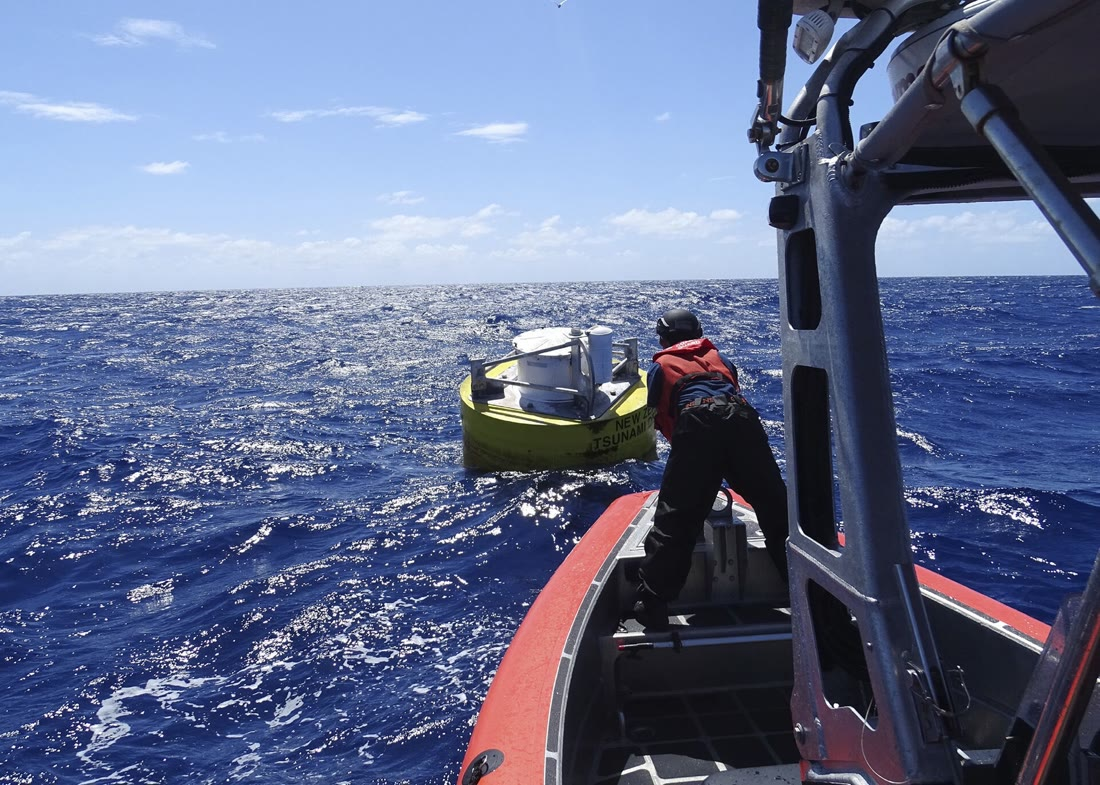
\includegraphics[width=\linewidth]{images/book1/g9-dart-buoy.jpg}
\end{minipage}\hfill
\begin{minipage}[c]{0.56\linewidth}\raggedright
{\small Um tripulante de um navio da Guarda Costeira dos Estados Unidos
inspeciona uma boia de alerta de \omterm{def:g7:earthquakes:tsunami}{tsunami} no \omterm{def:g2:water-on-earth:ocean}{oceano} Pacífico, em novembro
de 2021. A boia flutua acima de um registrador de pressão no fundo do
\omterm{def:g2:water-on-earth:ocean}{mar}, milhares de metros abaixo. U.S. Coast Guard (domínio público, via
Wikimedia Commons).}
\end{minipage}
% ledger: commons:dart-buoy
\label{fig:g9:natural-risks:buoy}
\end{omfigure}

\begin{history}[Uma rede de boias]
Em 2001, a primeira série de seis estações desse tipo ficou completa, no
\omterm{def:g2:water-on-earth:ocean}{oceano} Pacífico. Depois do \omterm{def:g7:earthquakes:tsunami}{tsunami} de dezembro de 2004, que atingiu os
\omterm{def:g1:landscapes-around-us:water}{litorais} do \omterm{def:g2:water-on-earth:ocean}{oceano} Índico sem nenhum sistema de alerta instalado
(\cref{ch:g7:earthquakes}), a rede cresceu: em março de 2008, havia 39
estações.
\end{history}
% ledger: ndbc:dart

Um alerta só salva vidas se chegar a pessoas que sabem o que fazer com
ele: os caminhos até um terreno mais alto estão sinalizados e treinados,
o kit de emergência está pronto, as escolas fazem simulados. Em Armero, a
ameaça era conhecida e o \omterm{def:g2:drawing-to-map:map}{mapa} estava desenhado; o alerta nunca chegou à
cidade.
% ledger: ready:kit, usgs:armero

\section{Exercícios}

\begin{exercise}[$\star$]\label{exo:g9:natural-risks:1}
Ameaça ou \omterm{def:g9:natural-risks:vulnerability}{vulnerabilidade}? (a) Um \omterm{def:g1:landscapes-around-us:water}{rio} que transborda quase toda
primavera. (b) Uma vila sem sistema de alerta. (c) Casas pesadas de
tijolo sem estrutura. (d) Um forte \omterm{def:g4:volcanoes-earthquakes-first-look:earthquake}{terremoto} numa \omterm{def:g7:earthquakes:fault}{falha} próxima. (e) Uma
cidade construída na saída de um \omterm{def:g1:landscapes-around-us:landform}{vale} por onde já desceram fluxos de
lama.
\end{exercise}

\begin{exercise}[$\star$]\label{exo:g9:natural-risks:2}
Verdadeiro ou falso? Corrija as frases falsas. (a) Uma \omterm{def:g5:natural-hazards:hazard}{ameaça natural} num
lugar onde ninguém mora é um \omterm{def:g9:natural-risks:risk}{risco} alto. (b) A \omterm{def:g9:natural-risks:prevention}{prevenção} pode reduzir a
\omterm{def:g9:natural-risks:vulnerability}{vulnerabilidade} de uma cidade. (c) Um \omterm{def:g9:natural-risks:hazard-map}{mapa de ameaças} mostra onde uma
ameaça pode atingir. (d) Um bom sistema de alerta torna um \omterm{def:g4:volcanoes-earthquakes-first-look:volcano}{vulcão} menos
perigoso.
\end{exercise}

\begin{exercise}[$\star$]\label{exo:g9:natural-risks:3}
Para cada ameaça, diga se ela pode ser prevista com dias ou horas de
antecedência: (a) uma \omterm{def:g5:natural-hazards:storm}{tempestade}; (b) uma \omterm{def:g5:water-shapes-the-land:flood}{inundação} depois de uma \omterm{def:g4:clouds-rain-snow:precipitation}{chuva}
forte; (c) um \omterm{def:g4:volcanoes-earthquakes-first-look:earthquake}{terremoto}; (d) a chegada de um \omterm{def:g7:earthquakes:tsunami}{tsunami} a um \omterm{def:g1:landscapes-around-us:water}{litoral} longe
de onde ele começou.
\end{exercise}

\begin{exercise}[$\star$]\label{exo:g9:natural-risks:4}
% ledger: usgs:hvo-toolkit
Use o desenho de um \omterm{def:g4:volcanoes-earthquakes-first-look:volcano}{vulcão} vigiado. O que cada instrumento mede, e que
sinal de alerta de uma \omterm{def:g4:volcanoes-earthquakes-first-look:eruption}{erupção} ele vigia? (a) Um \omterm{def:g7:earthquakes:seismometer}{sismômetro}. (b) Um
inclinômetro. (c) Um receptor GPS. (d) Um medidor de gases.
\end{exercise}

\begin{exercise}[$\star\star$]\label{exo:g9:natural-risks:5}
% ledger: usgs:armero
Em 1985, os fluxos de lama do Nevado del Ruiz chegaram a Armero, a
\qty{45}{km} de distância, cerca de duas horas depois da \omterm{def:g4:volcanoes-earthquakes-first-look:eruption}{erupção}. (a)
Qual foi a sua velocidade média, em quilômetros por hora? (b) Uma pessoa
anda a cerca de \qty{4}{km/h}. Que distância os moradores poderiam ter
percorrido a pé em duas horas? (c) Por que eles não saíram? (d) Dê duas
coisas que poderiam tê-los salvado.
\end{exercise}

\begin{exercise}[$\star\star$]\label{exo:g9:natural-risks:6}
% ledger: (invented region: figdata/grade-9/flood_zone.py)
Use o \omterm{def:g2:drawing-to-map:map}{mapa} das zonas de \omterm{def:g5:water-shapes-the-land:flood}{inundação} das Colinas de Varden. (a) Qual
\omterm{def:g5:water-shapes-the-land:flood}{inundação} cobre a faixa mais larga? (b) Com a quadrícula do \omterm{def:g2:drawing-to-map:map}{mapa}, meça a
largura de cada zona, de um lado ao outro do \omterm{def:g1:landscapes-around-us:landform}{vale}, a \qty{5}{km} leste.
(c) Um celeiro fica num terreno \qty{6}{m} acima do \omterm{def:g1:landscapes-around-us:water}{rio}.
Quais das três \omterm{def:g5:water-shapes-the-land:flood}{inundações} o alcançam? (d) Por que a \omterm{def:g5:water-shapes-the-land:flood}{inundação} \qty{2}{m}
acima do \omterm{def:g1:landscapes-around-us:water}{rio} é a que vem com mais frequência?
\end{exercise}

\begin{exercise}[$\star\star$]\label{exo:g9:natural-risks:7}
Coloque cada situação na grade do \omterm{def:g9:natural-risks:risk}{risco} (ameaça baixa ou alta,
\omterm{def:g9:natural-risks:vulnerability}{vulnerabilidade} baixa ou alta) e diga se o \omterm{def:g9:natural-risks:risk}{risco} é baixo, moderado ou
alto. (a) Prédios sólidos e simulados numa cidade sobre uma \omterm{def:g7:earthquakes:fault}{falha} ativa.
(b) Uma área de camping na \omterm{def:g5:water-shapes-the-land:flood}{planície de inundação} de um \omterm{def:g1:landscapes-around-us:water}{rio} que raramente
transborda. (c) Uma vila de casas frágeis ao pé de um \omterm{def:g4:volcanoes-earthquakes-first-look:volcano}{vulcão} ativo, sem
observatório. (d) Uma cidade no alto de um morro, longe de qualquer
\omterm{def:g7:earthquakes:fault}{falha}, \omterm{def:g1:landscapes-around-us:water}{rio} ou \omterm{def:g4:volcanoes-earthquakes-first-look:volcano}{vulcão}.
\end{exercise}

\begin{exercise}[$\star\star$]\label{exo:g9:natural-risks:8}
% ledger: iris:better-wall, explo:base-isolation
Três escolas são construídas no mesmo terreno. A escola A é uma estrutura
de pilares e vigas com paredes de tijolo entre eles; a escola B tem a
mesma estrutura, com travas diagonais e duas paredes de contraventamento;
a escola C tem a estrutura da B, apoiada sobre isoladores. (a) Classifique
as escolas da mais segura à menos segura num \omterm{def:g4:volcanoes-earthquakes-first-look:earthquake}{terremoto}. (b) Explique o
que as travas fazem. (c) Explique o que os isoladores fazem.
\end{exercise}

\begin{exercise}[$\star\star$]\label{exo:g9:natural-risks:9}
% ledger: fema:flood-zones
Um \omterm{def:g2:drawing-to-map:map}{mapa} de \omterm{def:g5:water-shapes-the-land:flood}{inundação} mostra a \omterm{def:g5:water-shapes-the-land:flood}{inundação} de 100 anos, que tem uma chance
de 1 em 100 de ser atingida ou ultrapassada num ano qualquer. (a)
Escreva essa chance como porcentagem. (b) Um vizinho diz: ``A \omterm{def:g5:water-shapes-the-land:flood}{inundação}
de 100 anos veio no ano passado, então estamos seguros por 99 anos.'' O
que está errado? (c) Em média, quantas \omterm{def:g5:water-shapes-the-land:flood}{inundações} desse tipo viriam em
300 anos?
\end{exercise}

\begin{exercise}[$\star\star$]\label{exo:g9:natural-risks:10}
% ledger: ndbc:dart, nws:tsunami-speed
Uma estação de alerta de \omterm{def:g7:earthquakes:tsunami}{tsunami} lê a pressão do fundo do \omterm{def:g2:water-on-earth:ocean}{mar} a cada
\qty{15}{s}. (a) Quantas leituras ela faz em uma hora? (b) Em um ano de
365 dias? Escreva a resposta em notação científica. (c) Um \omterm{def:g7:earthquakes:tsunami}{tsunami}
atravessa o \omterm{def:g2:water-on-earth:ocean}{oceano} profundo a cerca de \qty{800}{km/h}. Quanto tempo ele
leva para chegar a um \omterm{def:g1:landscapes-around-us:water}{litoral} a \qty{2400}{km} de distância? (d) Por que
esse tempo importa?
\end{exercise}

\begin{exercise}[$\star\star\star$]\label{exo:g9:natural-risks:11}
% ledger: ready:kit
Uma família de quatro pessoas prepara um kit de emergência com água para
3 dias, a cerca de \qty{3.8}{L} por pessoa por dia, para beber e se
lavar. (a) De quantos litros de água ela precisa? (b) Quantas garrafas de
\qty{1.5}{L} são? (c) Cite quatro outras coisas que o kit contém, e diga
por que cada uma é útil. (d) Por que o kit fica perto da porta?
\end{exercise}

\begin{exercise}[$\star\star\star$]\label{exo:g9:natural-risks:12}
% ledger: usgs:armero, usgs:hvo-toolkit
Uma cidade fica ao lado de um \omterm{def:g1:landscapes-around-us:water}{rio}, na saída de um \omterm{def:g1:landscapes-around-us:landform}{vale} que desce de um
\omterm{def:g4:volcanoes-earthquakes-first-look:volcano}{vulcão} nevado. Antigos depósitos de fluxos de lama ficam embaixo das suas
ruas. O \omterm{def:g4:volcanoes-earthquakes-first-look:volcano}{vulcão} começou a tremer com pequenos \omterm{def:g4:volcanoes-earthquakes-first-look:earthquake}{terremotos}. Escreva um plano
de \omterm{def:g9:natural-risks:prevention}{prevenção} de cinco pontos para a cidade. Para cada ponto, diga se ele
age do lado da ameaça (conhecer e vigiar a ameaça) ou do lado da
\omterm{def:g9:natural-risks:vulnerability}{vulnerabilidade} no \omterm{def:g9:natural-risks:risk}{risco}.
\end{exercise}

\section{Problema: Onde construir a nova escola?}

\begin{problem}[{Problema de fim de semana --- uma nova escola é posta
no mapa das Colinas de Varden, longe das inundações, das encostas
íngremes e da falha; a resposta final é o número de casas dentro da zona
de inundação}]
\label{pb:g9:natural-risks:1}
% ledger: (invented region: figdata/grade-9/flood_zone.py: sites A, B, C; 17 of 28 houses in the 5 m zone)
A vila das Colinas de Varden precisa de uma nova escola, e três terrenos
são oferecidos: A, B e C, no \omterm{def:g2:drawing-to-map:map}{mapa} abaixo. A zona de \omterm{def:g5:water-shapes-the-land:flood}{inundação} sombreada
no \omterm{def:g2:drawing-to-map:map}{mapa} é todo o terreno a menos de \qty{5}{m} acima do \omterm{def:g1:landscapes-around-us:water}{rio}, que uma
grande \omterm{def:g5:water-shapes-the-land:flood}{inundação} cobriria. A tabela dá, para cada terreno, a \omterm{def:g4:world-physical-map:altitude}{altitude} do
chão, o nível do \omterm{def:g1:landscapes-around-us:water}{rio} ao lado e quanto o chão sobe em \qty{200}{m}
medidos na horizontal, através da encosta.

\begin{center}
{\small
\begin{tabular}{|c|c|c|c|}
\hline
terreno & \omterm{def:g4:world-physical-map:altitude}{altitude} do chão & nível do \omterm{def:g1:landscapes-around-us:water}{rio} ao lado & subida do chão em \qty{200}{m} \\
\hline
A & \qty{137}{m} & \qty{137}{m} & \qty{1.4}{m} \\
B & \qty{276}{m} & \qty{126}{m} & \qty{83}{m} \\
C & \qty{236}{m} & \qty{143}{m} & \qty{20}{m} \\
\hline
\end{tabular}}
\end{center}

\begin{omfigure}
\begin{tikzpicture}
\begin{axis}[axis equal image, xmin=3.5, xmax=7, ymin=2.7, ymax=5.5, width=11.5cm,
  enlargelimits=false, tick label style={font=\scriptsize}, xlabel={leste (km)},
  ylabel={norte (km)}, label style={font=\small}, xtick={3.5,4,...,7}, ytick={3,3.5,...,5.5}]
\addplot[contour] table {figdata/out/grade-9-flood_zone-contours.dat};
\addplot[index contour] table {figdata/out/grade-9-flood_zone-index.dat};
\addplot[fill=blue!25, draw=blue!50, line width=0.3pt] table {figdata/out/grade-9-flood_zone-zone.dat} -- cycle;
\addplot[only marks, mark=none, point meta=explicit symbolic, nodes near coords,
  nodes near coords align={center}, nodes near coords style={font=\tiny, fill=white, inner sep=0.6pt, text=omContour}]
  table[meta=z] {figdata/out/grade-9-flood_zone-index-lab.dat};
\addplot[river] table {figdata/out/grade-9-flood_zone-river.dat};
\addplot[fault] table {figdata/out/shared-region-fault.dat};
\addplot[only marks, mark=square*, mark size=1.5pt, mark options={fill=black}] table {figdata/out/grade-9-flood_zone-houses-in.dat};
\addplot[only marks, mark=square*, mark size=1.5pt, mark options={fill=black}] table {figdata/out/grade-9-flood_zone-houses-out.dat};
\addplot[only marks, mark=*, mark size=2.6pt, mark options={fill=omWarm, draw=black}, point meta=explicit symbolic,
  nodes near coords, nodes near coords align={anchor=south west},
  nodes near coords style={font=\small\bfseries, fill=white, inner sep=1pt, xshift=2.5pt, yshift=2.5pt}]
  table[meta=name] {figdata/out/grade-9-flood_zone-sites.dat};
\node[font=\footnotesize, fill=white, inner sep=1pt, anchor=west] at (axis cs:6.42,5.05) {falha};
\coordinate (na) at (axis cs:3.7,4.75);
\fill[black] (axis cs:5.8,2.85) rectangle (axis cs:5.925,2.9);
\fill[white] (axis cs:5.925,2.85) rectangle (axis cs:6.05,2.9);
\fill[black] (axis cs:6.05,2.85) rectangle (axis cs:6.175,2.9);
\fill[white] (axis cs:6.175,2.85) rectangle (axis cs:6.3,2.9);
\draw[black, line width=0.4pt] (axis cs:5.8,2.85) rectangle (axis cs:6.3,2.9);
\node[font=\footnotesize, above, inner sep=1.5pt, fill=white] at (axis cs:6.05,2.9) {\qty{500}{m}};
\end{axis}
\fill[white, opacity=0.85] ($(na)+(-0.35,-0.1)$) rectangle ($(na)+(0.35,1.45)$);
\pic at (na) {northarrow};
\end{tikzpicture}

{\small A vila, os três terrenos para a escola e a zona de \omterm{def:g5:water-shapes-the-land:flood}{inundação}
(sombreada), no \omterm{def:g2:drawing-to-map:map}{mapa} das Colinas de Varden (linhas finas de mesma altura
a cada \qty{10}{m}). Cada pequeno quadrado preto é uma casa. A linha
preta grossa é uma \omterm{def:g7:earthquakes:fault}{falha}.}
\label{fig:g9:natural-risks:school-map}
\end{omfigure}

\noindent\textbf{Parte I --- A zona de inundação.}\par\nopagebreak
\begin{enumerate}[beginpenalty=10000]
  \item Usando os níveis do \omterm{def:g1:landscapes-around-us:water}{rio} da tabela, diga em que sentido o \omterm{def:g1:landscapes-around-us:water}{rio}
        corre.
  \item Calcule a altura de cada terreno acima do \omterm{def:g1:landscapes-around-us:water}{rio} ao seu lado.
  \item Qual dos três terrenos fica na zona de \omterm{def:g5:water-shapes-the-land:flood}{inundação}?
  \item Use a \omterm{def:g2:drawing-to-map:scale}{escala} gráfica para medir a largura da zona de \omterm{def:g5:water-shapes-the-land:flood}{inundação},
        de um lado ao outro do \omterm{def:g1:landscapes-around-us:landform}{vale}, no terreno A.
\end{enumerate}

\noindent\textbf{Parte II --- As encostas e a falha.}\par\nopagebreak
\begin{enumerate}[resume, beginpenalty=10000]
  \item A declividade em porcentagem é a subida do chão para cada
        \qty{100}{m} medidos na horizontal. Calcule a declividade em cada
        terreno.
  \item Qual terreno ficaria exposto a um \omterm{def:g5:natural-hazards:landslide}{deslizamento de terra}? Explique.
  \item Use a \omterm{def:g2:drawing-to-map:scale}{escala} gráfica para estimar a distância de cada terreno à
        \omterm{def:g7:earthquakes:fault}{falha}.
  \item Suponha que a \omterm{def:g7:earthquakes:fault}{falha} ainda possa se mover. Por que o chão bem em
        cima dela é um mau lugar para uma escola?
\end{enumerate}

\noindent\textbf{Parte III --- Escolher.}\par\nopagebreak
\begin{enumerate}[resume, beginpenalty=10000]
  \item Desenhe uma tabela com uma linha por terreno e três colunas: na
        zona de \omterm{def:g5:water-shapes-the-land:flood}{inundação}? encosta íngreme? sobre a \omterm{def:g7:earthquakes:fault}{falha}? Preencha com
        sim ou não.
  \item Qual terreno você escolheria? Justifique a sua escolha com a
        tabela.
  \item O terreno escolhido ainda fica numa região onde o chão pode
        tremer. Cite duas maneiras de construir a escola, e um hábito dos
        seus alunos, que reduzem a sua \omterm{def:g9:natural-risks:vulnerability}{vulnerabilidade}.
  \item A escola também vai servir de abrigo durante as \omterm{def:g5:water-shapes-the-land:flood}{inundações}. Conte
        as casas da vila que ficam dentro da zona de \omterm{def:g5:water-shapes-the-land:flood}{inundação}. Que fração
        de todas as casas isso representa?
\end{enumerate}
\end{problem}
